\documentclass[sigconf]{acmart}

\usepackage{graphicx,url}
\usepackage[utf8]{inputenc}
\usepackage[english]{babel}
\usepackage{xcolor}
\usepackage{cleveref}
\usepackage{listings}

% ADD SUBSUBSUBSECTION
\newcommand{\subsubsubsection}[1]{\paragraph{#1}\mbox{}\\}
\setcounter{secnumdepth}{4}
\setcounter{tocdepth}{4}


%%
%% \BibTeX command to typeset BibTeX logo in the docs
\AtBeginDocument{%
  \providecommand\BibTeX{{%
    \normalfont B\kern-0.5em{\scshape i\kern-0.25em b}\kern-0.8em\TeX}}}

%% Rights management information.  This information is sent to you
%% when you complete the rights form.  These commands have SAMPLE
%% values in them; it is your responsibility as an author to replace
%% the commands and values with those provided to you when you
%% complete the rights form.
\setcopyright{acmcopyright}
\copyrightyear{2018}
\acmYear{2018}
\acmDOI{10.1145/1122445.1122456}

%% These commands are for a PROCEEDINGS abstract or paper.
\acmConference[Woodstock '18]{Woodstock '18: ACM Symposium on Neural
  Gaze Detection}{June 03--05, 2018}{Woodstock, NY}
\acmBooktitle{Woodstock '18: ACM Symposium on Neural Gaze Detection,
  June 03--05, 2018, Woodstock, NY}
\acmPrice{15.00}
\acmISBN{978-1-4503-XXXX-X/18/06}


%%
%% Submission ID.
%% Use this when submitting an article to a sponsored event. You'll
%% receive a unique submission ID from the organizers
%% of the event, and this ID should be used as the parameter to this command.
%%\acmSubmissionID{123-A56-BU3}

%%
%% The majority of ACM publications use numbered citations and
%% references.  The command \citestyle{authoryear} switches to the
%% "author year" style.
%%
%% If you are preparing content for an event
%% sponsored by ACM SIGGRAPH, you must use the "author year" style of
%% citations and references.
%% Uncommenting
%% the next command will enable that style.
%%\citestyle{acmauthoryear}

%%
%% end of the preamble, start of the body of the document source.
\begin{document}

%%
%% The "title" command has an optional parameter,
%% allowing the author to define a "short title" to be used in page headers.
\title{Garm: A Blockchain based platform for supply chain management}

%%
%% The "author" command and its associated commands are used to define
%% the authors and their affiliations.
%% Of note is the shared affiliation of the first two authors, and the
%% "authornote" and "authornotemark" commands
%% used to denote shared contribution to the research.
\author{Edivaldo M. F. J. Júnior}
\email{edivaldojunior@ifba.edu.br}
\affiliation{%
  \institution{Instituto Federal da Bahia (IFBA)}
  \streetaddress{Rua Emídio dos Santos, S/N}
  \city{Salvador}
  \state{Bahia}
  \country{Brazil}
  \postcode{40301-015}
}

\author{Manoel C. M. Neto}
\email{manoelnetom@ifba.edu.br}
\affiliation{%
  \institution{Instituto Federal da Bahia (IFBA)}
  \streetaddress{Rua Emídio dos Santos, S/N}
  \city{Salvador}
  \state{Bahia}
  \country{Brazil}
  \postcode{40301-015}
}

\author{Allan E. S. Freitas}
\email{allan@ifba.edu.br}
\affiliation{%
  \institution{Instituto Federal da Bahia (IFBA)}
  \streetaddress{Rua Emídio dos Santos, S/N}
  \city{Salvador}
  \state{Bahia}
  \country{Brazil}
  \postcode{40301-015}
}

%%
%% By default, the full list of authors will be used in the page
%% headers. Often, this list is too long, and will overlap
%% other information printed in the page headers. This command allows
%% the author to define a more concise list
%% of authors' names for this purpose.
%\renewcommand{\shortauthors}{Trovato and Tobin, et al.}

%%
%% The abstract is a short summary of the work to be presented in the
%% article.
\begin{abstract}
  A complex web of relationships provides goods for manufacturing, assembling and delivering of final products known as supply chain. Emerging technologies have been used in supply chain systems in order to provide traceability. However, these systems tend to be centralized, monopolistic, asymmetric and opaque. As a consequence, these systems may result in trusting problems, such as fraud, corruption and tampering. Blockchain technology provides a new approach for information systems based on decentralization, that can apply for these supply chain systems. This work presents a Blockchain-based platform for developing applications that provide such traceability for the supply chain management. 
\end{abstract}

%%
%% The code below is generated by the tool at http://dl.acm.org/ccs.cfm.
%% Please copy and paste the code instead of the example below.
%%
\begin{CCSXML}
<ccs2012>
 <concept>
  <concept_id>10010520.10010553.10010562</concept_id>
  <concept_desc>Computer systems organization~Embedded systems</concept_desc>
  <concept_significance>500</concept_significance>
 </concept>
 <concept>
  <concept_id>10010520.10010575.10010755</concept_id>
  <concept_desc>Computer systems organization~Redundancy</concept_desc>
  <concept_significance>300</concept_significance>
 </concept>
 <concept>
  <concept_id>10010520.10010553.10010554</concept_id>
  <concept_desc>Computer systems organization~Robotics</concept_desc>
  <concept_significance>100</concept_significance>
 </concept>
 <concept>
  <concept_id>10003033.10003083.10003095</concept_id>
  <concept_desc>Networks~Network reliability</concept_desc>
  <concept_significance>100</concept_significance>
 </concept>
</ccs2012>
\end{CCSXML}

\ccsdesc[500]{Computer systems organization~Embedded systems}
\ccsdesc[300]{Computer systems organization~Redundancy}
\ccsdesc{Computer systems organization~Robotics}
\ccsdesc[100]{Networks~Network reliability}

%%
%% Keywords. The author(s) should pick words that accurately describe
%% the work being presented. Separate the keywords with commas.
\keywords{Blockchain, supply chain management, traceability, smart contracts}

%% A "teaser" image appears between the author and affiliation
%% information and the body of the document, and typically spans the
%% page.
%\begin{teaserfigure}
%  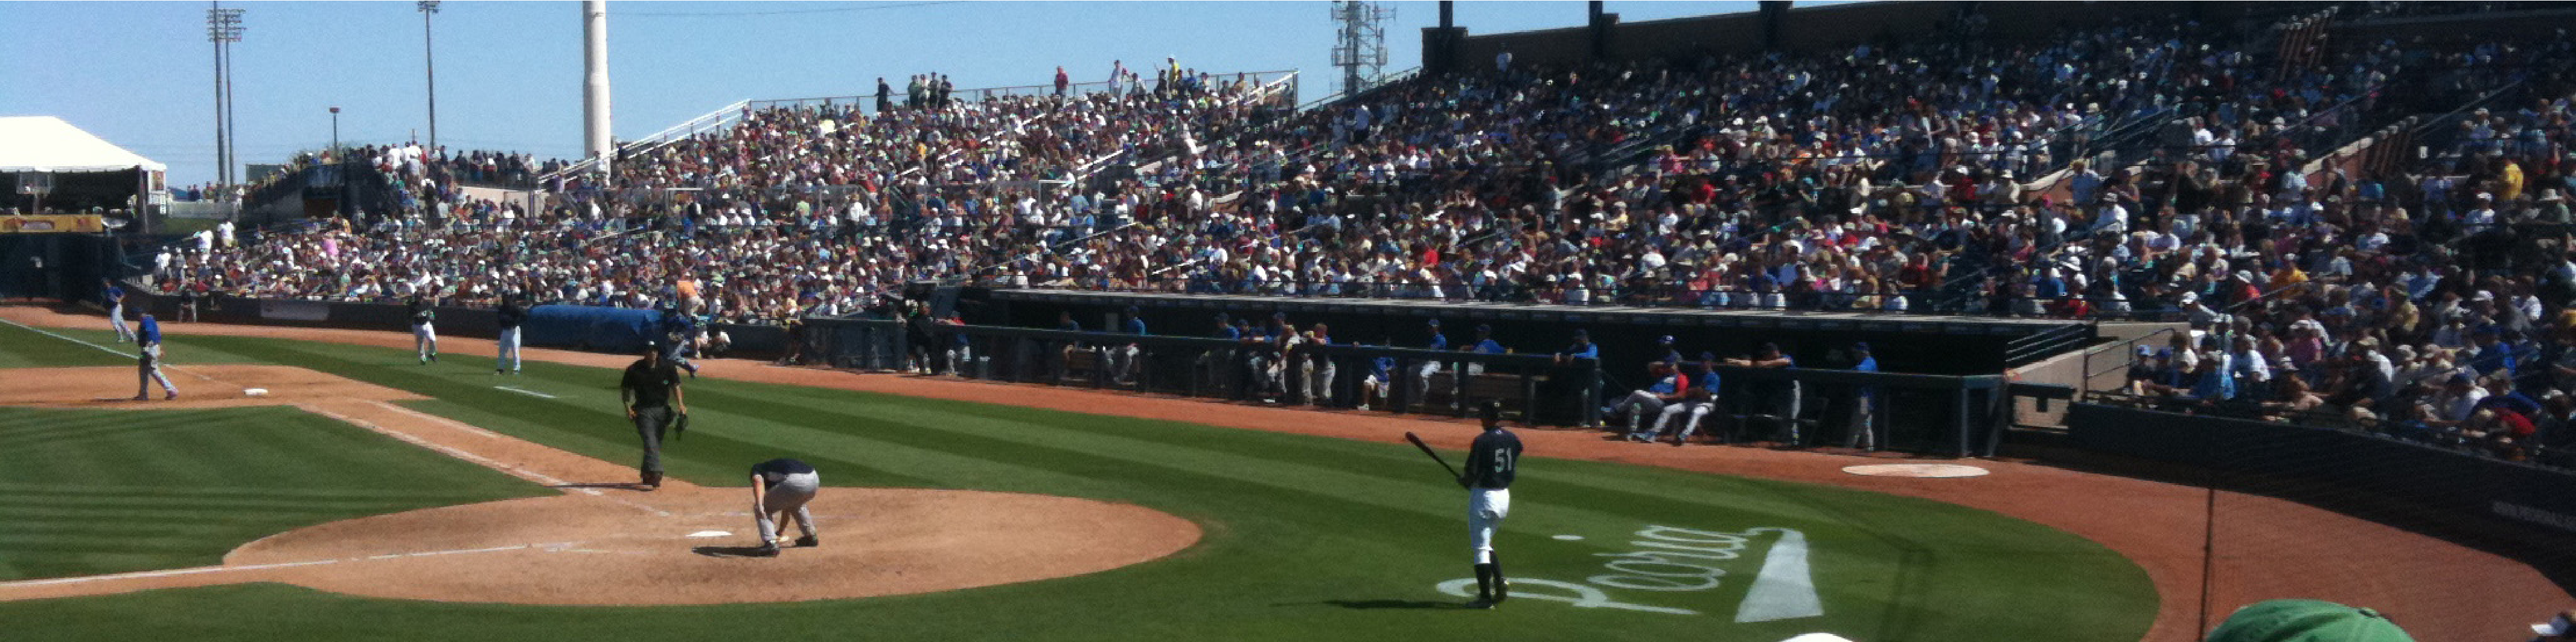
\includegraphics[width=\textwidth]{sampleteaser}
%  \caption{Seattle Mariners at Spring Training, 2010.}
%  \Description{Enjoying the baseball game from the third-base
%  seats. Ichiro Suzuki preparing to bat.}
%  \label{fig:teaser}
%\end{teaserfigure}

%%
%% This command processes the author and affiliation and title
%% information and builds the first part of the formatted document.
\maketitle

\textcolor{red}{O QUE COLOCAR EM CCS CONCEPTS}

\section{Introduction} \label{sec:Introduction}

Hundreds of years ago, supply chains were fairly simple. Mines and farms provided natural resources to skilled craftsman like blacksmiths and tailors who then created and sold goods. Nowadays, supply chains are much more complicated, fragmented and difficult to understand. Most of the time, the various companies don't know about each other and a final consumer likely don't know anything about how, where, when or under what condition the products passed through. This isn't just a problem for consumers. Today's supply chains are so complex that even big industry players have difficulty tracking how their goods get made \cite{swan2015blockchain}.

%{\color{red}adicionar aqui texto sobre o problema atual da cadeia de suprimento.}

In order to solve some problems that come with this complexity, such as supply chain visibility and traceability, many systems have been developed. However, these systems typically store information in standard databases controlled by service providers. This centralized data storage becomes a single point of failure and risks tampering. As a centralized organization, it can become a vulnerable target for bribery, and then the whole system can not be trusted anymore \cite{tian2017supply}.

Blockchain and smart contracts could make supply chain management simpler and more transparent. The idea is to create a single source of information about products and supply chain via global ledger. Each component would have its own entry on the blockchain that gets tracked over time. Both untrust companies could then update the status of a good in real-time. The end result is once the clients receive their products they could track every piece back to its manufacturer \cite{greve2018blockchain}.

Companies can also use the blockchain supply chain as a single source of truth for their products. They can manage and monitor risks within the supply chain, ensure quality of delivery and track the status of all components. Additionally companies can use smart contracts to manage and pay for supply chain autonomously \cite{tian2017supply}. 

This would reduce the need for large contract invoices on the back-and-forth of refund requests for faulty components. Those same smart contracts could assist with shipping and logistics tracking valuable products as they travel around the world. Companies using blockchain can finally have a complete picture of their products at every stage in the supply chain, bringing transparency to the production process while reducing the cost of manufactured goods  \cite{swan2015blockchain}.

This work presents Árion, a generic framework intended to be used in any kind of supply chain correlated to assets and products.
\section{Blockchain} \label{sec:Theoretical}

%\subsubsubsection

%\input{chapters/2_THEORETICAL_BACKGROUND/sections/1_blockchain.tex}
%\input{chapters/2_THEORETICAL_BACKGROUND/sections/2_fundamentalsOfBlockchain.tex}
%\input{chapters/2_THEORETICAL_BACKGROUND/sections/4_smartContracts.tex} 
%\input{chapters/2_THEORETICAL_BACKGROUND/sections/5_traceability.tex}

%%%%%%%%%%%%%%%%%%%%%%%%%%%%%%%%%%%%%%%%%%%%%%
While the system of financial institutions that serve as third parties reliable processors for processing payments work well for most still suffers from the shortcomings inherent in the model based on confidence. In addition, the cost of mediation increases transaction costs, which limits the practical minimum size of the transaction and eliminates the possibility of small occasional transactions. To solve these problems, \cite{nakamoto2008bitcoin} defined an electronic payment system called Bitcoin, based on cryptographic proof rather than reliable, allowing either party willing to transact directly with each other without the need to a reliable third party. 

Blockchain can be considered as a public ledger, in which all committed transactions are stored in a block chain \cite{zheng2016blockchain}. For \cite{swan2015blockchain}, besides the currency ( "Blockchain 1.0"), smart contracts ("2.0") demonstrate how the Blockchain is in a position to become the fifth disruptive computing paradigm after mainframes, PCs, Internet and mobile/ social networks. Smart contracts mediate registering in public ledger through an application executed in Blockchain itself.

Blockchain technology has critical features, such as decentralization, persistence, anonymity and auditability. Blockchain can function in a decentralized environment that is activated by the integration of several key technologies such as cryptographic hash, digital signature and distributed consensus engine, significantly save the cost and improve efficiency \cite{zheng2016blockchain}.

%%%%%%%%%%%%%%%%%%%%%%%%%%%%%%%%%%%%%%%%%%%%%%

%\subsubsection{Cryptography}\label{sec:criptografia}
%Blockchain relies heavily on encryption to satisfy system and application security requirements. As the word suggests, cryptocurrencies also make heavy use of encryption. Encryption provides a mechanism for safely encoding the rules of a system encryption on the system itself. This can be used to prevent tampering and misconceptions. So, before be able to understand blockchains correctly, it is necessary to understand the cryptographic foundations \cite{narayanan2016bitcoin}. Cryptography is a deep academic field of research that uses many advanced mathematical techniques that are notoriously subtle and complicated \cite{narayanan2016bitcoin}.

%\subsubsubsection{Cryptographic Hashes}\label{sec:hashesCriptograficos}
%Hash is a mathematical function that converts any form of data into a unique string of text with the three properties to be follow \cite{narayanan2016bitcoin}:

%\begin{itemize}
%\item  Its input can be any string of any length;
%\item Produces a fixed size output (eg., 256 digits);
%\item It is efficiently computable. Technically, hashing a n-bit string must have a $O(n)$ runtime.
%\end{itemize}

%These properties define a general hash function. Cryptographic hash functions are unidirectional and hardly allow retrieving the original value $x$ from the hash $h$. For a hash function to be cryptographically safe, it must satisfy the following three properties: (1) collision resistance, (2) hiding and (3) puzzle friendliness \cite{greve2018blockchain}.

%A collision occurs when two distinct inputs produce the same output. A hash function $H$ is collision resistant when it is impossible to find two values $x$ and $y$ such that $x \neq y$ and $H(x) = H(y)$ \cite{narayanan2016bitcoin}.

%The hide property states that, having the hash function output $y = H (x)$, there is no possible way to find out which was the $x$ input \cite{greve2018blockchain}.

%A hash function $H$ is considered puzzle friendliness if for each possible output value of $n$ bits $y$ if $k$ is chosen from a distribution with high min-entropy, then it is impracticable to find $x$ such that $H (k \| x) = y$ in time significantly less than $2^n$ \cite{narayanan2016bitcoin}.

%\subsubsubsection{Digital Signatures}\label{sec:assinaturasDigitais}
%A digital signature is supposed to be a digital analog of a handwritten paper signature. Two signature properties are desired which correspond well to the analogy of the handwritten signature: first, only one person can make their own signature, but anyone can verify if it is valid. Secondly, it is desired that the signature must be linked to a specific document, so the signature cannot be used to indicate the agreement or endorsement to a different document \cite{merkle1989certified}. Moreover, it is not possible to forge a signature in such a way as to reuse it in some other context. That is, signatures must be irrefutable.

%To implement digital signatures, asymmetric key encryption is used. A secret key (sk) is used for signing the document and a public key (pk) is used to attest the signature's authenticity. A digital signature consists of the following algorithms \cite{greve2018blockchain}:

%\begin{itemize}
%\item $(sk , pk) := generateKeys(keysize)$ – The $generateKeys()$ method receives a key size $(keysize)$ in the input and return a pair of public $(pk)$ and private $(sk)$ keys.
%\item $sig := sign(sk , msg)$ – The method $sign()$ receives a message $msg$ and a secret key $(sk)$ on entry and returns the signature $sig$ f that message under $sk$.
%\item $isValid := veri f y(pk , msg , sig)$ – The method $verify$ receives a public key $(pk)$, a message $msg$ and a signature $(sig)$ as input, and returns a boolean value: $isValid = true$ if $sig$ is a signature valid for $msg$ under $pk$; $isValid = false$, otherwise.
%\end{itemize}

%The following two properties must be maintained:

%\begin{itemize}
%\item Authenticity: Signatures can be validated: \\ $verify(pk, message, sign(sk, message)) = = true$.
%\item Signatures are existentially unfalsifiable: signature cannot be forged.
%\end{itemize}

%It is noted that \textit{generateKeys()} and \textit{sign()} can be random algorithms. In fact, generating keys should be randomized, because it should be generating different keys for different people. On the other hand, \textit{verify()} will always be deterministic \cite{greve2018blockchain}.

%\subsubsection{Consensus}\label{sec:consenso}
%The key to blockchain operation is that the network must agree collectively on the ledger's content. Instead of a central entity maintain control over information (such as a bank for example), the data is shared among all. This requires the network to maintain the consensus around the information recorded in the block chain. How this consensus is reached, affects the security and economic parameters of the protocol \cite{kostarev2017review}.

%Reaching consensus is a challenge for blockchain, because its network is distributed and there is no central node that ensures that ledgers on distributed nodes be all the same. Nodes do not need to trust other nodes. Thus, protocols are required to ensure that ledgers on different nodes are consistent \cite{kostarev2017review}. A good consensus algorithm means efficiency, security and convenience. Current common consensus algorithms still have many shortcomings. New consensus algorithms are created to solve some blockchain-specific problems \cite{zheng2016blockchain}.

%\subsubsection{Distributed Ledger}\label{sec:livro}
%Distributed ledger is a data structure distributed by several nodes or computing devices. Each node replicates and saves a identical ledger copy. Each participating node in the network updates independently \cite{greve2018blockchain}.

%At the simplest level, a blockchain immutably records transactions which update states in a ledger. A smart contract programmatically accesses two distinct pieces of the ledger – a blockchain, which immutably records the history of all transactions, and a world state that holds a cache of the current value of these states, as it’s the current value of an object that is usually required \cite{zheng2016blockchain}.

%\subsubsubsection{Transactions}\label{sec:transac}
%Blockchain is a public digital book that records online transactions. The blockchain algorithm automatically graphs and authenticates the transaction, which is immediately visible to all users, minimizing the possibility of fraud \cite{Bankrate2018}.

%From a technical standpoint, the most fundamental definition of a transaction is an atomic event allowed by the underlying protocol. A transaction determines a sequence of state operations. It adds a transfer of asset or, generally speaking, a smart contract. In a basic case, the transaction girds a digital signature of the issuer holding the asset and the receiver's address, as well as inputs and outputs for transaction. Entries indicate the previous transaction hash which is related to the current one \cite{greve2018blockchain}.

%\subsubsubsection{Blocks}\label{sec:blocks}
%Blocks contains a header with information needed for current maintenance and its validation. A block consists of the block header and block body. The body's block consists of a transaction counter and transaction. The maximum number of transactions a block can hold depends on block size and the size of each transaction %\cite{zheng2016blockchain}.

%Validate a block consists in verifying (i) if its structure is well formed (ii) its hash is valid (meets the challenge), (iii) its size is within the network accepted limit, (iv) the set of transactions within the block is valid, (v) the first transaction (and only the first) is the coinbase transaction. The blocks are validated independently, by each node of the blockchain network, and this feature contributes to the process decentralization \cite{greve2018blockchain}.

\subsection{Public Blockchain Versus Private Blockchain}\label{sec:versus}
On a public blockchain, any person can participate without a specific identity. Public blockchains typically involve a native cryptocurrency and often use proof-of-work (PoW) consensus and economic incentives \cite{androulaki2018hyperledger}. Public blockchain can be audited by anyone, and each node has as much transmission power as any other. For a transaction to be considered valid, it must be authorized by all nodes constituents via the consensus process. As long as each node meets protocol-specific stipulations, their transactions can be validated and thus added to the chain \cite{greve2018blockchain}.

Private blockchains, on the other hand, perform a blockchain between a set of known and identified participants. A private blockchain provides a way to protect the interactions between a group of entities that have a common goal but that don't totally trust each other, like companies that trade funds, assets or information. Relying on peer identities, one private blockchain may use the traditional consensus of Byzantine fault tolerance (BFT) \cite{androulaki2018hyperledger}.

%%%%%%%%%%%%%%%%%%%%%%%%%%%%%%%%%%%%%%%%%%%%%%
\subsection{Smart Contracts}\label{sec:smartContracts}
A smart contract is a computerized transaction protocol that executes the terms of a contract \cite{szabo1997idea}. The term smart contract (SC) means: “an internal transaction protocol format that executes the terms of a contract. Their overall goals are ensure common contractual conditions, minimize malicious and accidental exceptions and the need for reliable intermediaries. Related economic objectives include reducing fraud losses, arbitration and execution costs, and other transaction costs.” \cite{szabo1997idea}.

Smart contracts are created as scripts, stored in with exclusive addressing on the Blockchain itself. They are triggered when addressing a transaction to it. Then the script is executed independently and automatically, as prescribed in all nodes in the network according to the data included in the transaction \cite{greve2018blockchain}. Smart contracts interpret the code objectively - "The Code is the law".




%%%%%%%%%%%%%%%%%%%%%%%%%%%%%%%%%%%%%%%%%%%%%%  
\section{Supply Chain Management} \label{sec:General}

Billions of products have being manufactured every day through complex supply chains that can extend to all parts of the world. However, tracing good flows from harvesting and manufacturing to the final consumer is hard. To achieve this flow, we need to improve Supply Chain visibility \cite{galvez2018future}. %Before reaching the end consumer, the goods go through an often wide network of retailers, distributors, carriers, warehousing facilities and suppliers who participate in the design, production, delivery and sales process of a product, but in many cases. These steps are a dimension invisible to the consumer \cite{provenance2015}.
%Traceability is the ability to preserve the product identities, their origins, and transformations, so that the collection, documentation and maintenance of information related to all processes in the production chain must be ensured \cite{gryna1998juran, Opara2001} .

Traceability is one of the key challenges encountered in the business world, with most companies having little or no information about their own second and third-tier suppliers. Transparency and end-to-end visibility of the supply chain can help shape product, raw material, test control, and end product flow, enabling better operations and risk analysis to ensure better chain productivity \cite{abeyratne2016blockchain}.

%inicio do general context antigo
Traceability systems typically store information in standard databases controlled by service providers. This centralized data storage becomes a single point of failure and tampering risks. As a consequence, these systems result in trusting problems, such as fraud, corruption and tampering. Likewise, as a single point of failure, a centralized system is vulnerable to collapse \cite{tian2017supply}.

Nowadays, Blockchain presents a whole new approach based on decentralization, enabling end-to-end traceability, allowing consumers to access the asset's history of these products through a software application \cite{galvez2018future}.

SCM requires to control who can write and read data to/from the Blockchain. In order to do that, the first step is identity. In the SCM context, the peers are known and the system needs to know who a user is, to define rules about what data they can commit, and what data they can consume from the ledger. So, in a corporate case scenario, Blockchain for the business, Blockchain for supply value chains, a private Blockchain provides this needed characteristic.
\section{Related Work} \label{sec:RelatedWork}

The rapid growth of internet technologies allowed the onset of lots of technologies applied in traceability systems. However, these systems tend to be centralized, monopolistic, and asymmetric. As a consequence, these systems result in trust problems, such as fraud, corruption, tampering, and falsifying information. Likewise, by being a single point of failure, a centralized system is vulnerable to collapse.

Blockchain presents a whole new approach based on decentralization. Nonetheless, by being in its early stages, it has some challenges to deal with, in which scalability and performance become mainly defiance to face the huge amount of data in the real world. Using this technology some solutions have been raised, as follows.

In order to solve some problems with Supply Chain traceability, many internet of things (IoT) technologies, such as RFID and wireless sensor network-based architectures has been applied. However these technologies doesn't guarantee that the information shared by supply chain members in the traceability systems can be trusted \cite{tian2017supply}.

In \cite{tian2017supply}, it is proposed a system that combines haccp (a food safety protocol), Blockchain and IoT in order to provide food safety traceability, involving suppliers, producers, manufacturers, distributors, retailers, consumers and certifiers. Each of these members can add, update and check the information about the product on the Blockchain as long as they register as a user in the system. Each product has also a unique digital cryptographic identifier that connects the physical items to their virtual identity in the system. This virtual identity can be seen as the product information profile.

There are advantages of applying the Blockchain concept to a supply chain. One of the most important is: all stakeholders involved in the supply chain are motivated by the need to demonstrate to customers the superior quality of their methods and products \cite{lu2017adaptable}. 

In addition to serving the functions of a traceability system, a Blockchain can be used as a marketing tool. As Blockchains are fully transparent and participants can control the assets in them, they can be used to enhance image and reputation of a company \cite{van2007essentials}, drive loyalty among existing customers \cite{pizzuti2015global} and attract new ones \cite{svensson2009transparency}. In fact, companies can easily distinguish themselves from competitors by emphasizing transparency and monitoring product flow along the chain. 

The Everledger Diamonds project provides a Blockchain based solution to facilitate tracking from mine to consumer, enabling easier compliance against increasingly strict measures from diamonds produced \cite{crosby2016blockchain}.

IBM Food Trust is a pilot project motivated by food contamination scandals worldwide. The main goal is to tackling food safety in the supply chain using Blockchain technology. This platform tracked pork in China and mangoes in the Americas \cite{kamath2018food}.

These projects are focused on specific products only and are closed projects. Still, there is a general lack of standards for implementation of a Blockchain approach for traceability. A Blockchain must be universal and adaptable to specific situations \cite{valenta2017comparison}. In addition, the need to agree on a particular type of Blockchain to be used puts the parties under pressure. 

Our work is intended to provide a Blockchain based framework in order to facilitate the development of applications for traceability in supply chain management.
\section{Proposed Framework} \label{sec:Technical}
The main objective of this work is to create a generic framework for Supply Chain Management (SCM). Árion project is divided into three main modules described below: Frond-End WebApp, Back-End WebApp and Data Storage. Figure~\ref{fig:detalhamentotecnico} shows the application architecture and its components.

A SCM platform relies on three main items: assets (the goods itself or a token related to it), steps (phases which products go through) and actors (people who transact assets during the steps). Our approach is based on this triad, that must be defined on creation of a new supply chain.

Initially, a configuration file in JSON format is generated and read in the Blockchain platform, adding the main information for the correct functioning of the chain. The mechanism for creating this configuration file is detailed in the Sections \Cref{sec:UserInteraction,sec:ServiceLayer}.

%htbp
\begin{figure*}[ht]
\begin{center}
  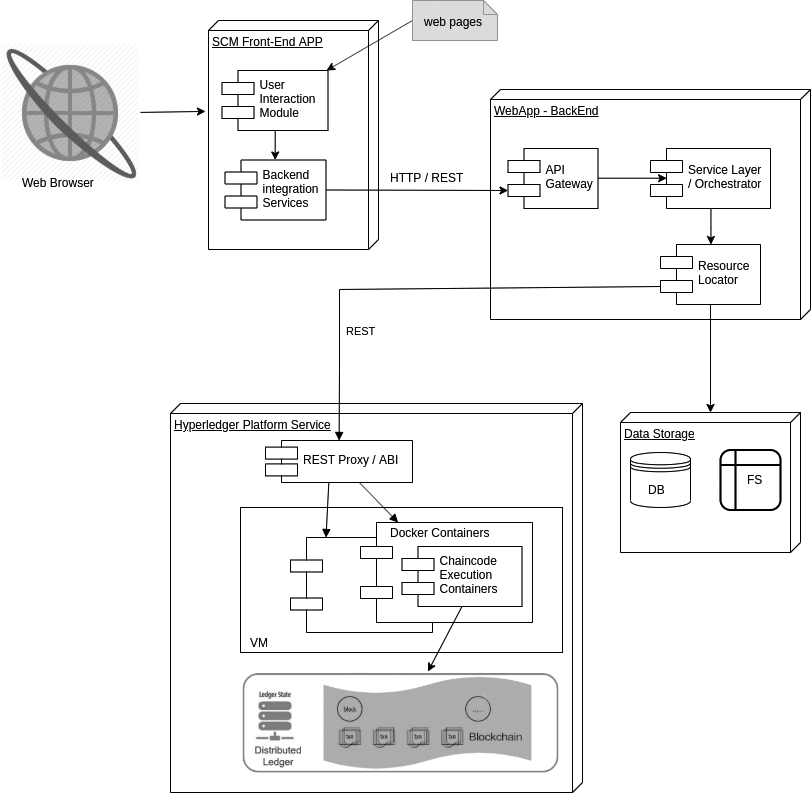
\includegraphics[scale=0.4]{images/detalhamentotecnico.png}
\caption{Árion Application architecture}
\label{fig:detalhamentotecnico}
\end{center}
\end{figure*}

\subsection{Frond-End WebApp}\label{sec:WebAppFrondEnd}
Front-End WebApp is a client–server application which the client (including the user interface and client-side logic) runs in a web browser. This is a single-page application (SPA) that interacts with the user by dynamically rewriting the current page rather than loading entire new pages from a server. The application is build with React (also known as React.js or ReactJS). The Front-End Webapp is divided into two main blocks and these are classified according to the interactions: User Interaction Modules and Backend Interaction Services.

\subsubsection{User Interaction Modules}\label{sec:UserInteraction}
User Interaction modules are responsible for providing web pages that will be rendered on client’s web browser. These interactions are provided by modules described below.

The Login Module is responsible for display the login and authentication alternatives pages (e.g. ‘forgot my password’, ‘reset my password’). The Application Configuration module provides the features of the creation/configuration of supply chain items and supply chain flows (steps). This module is responsible for getting the information from the user to generate the configuration JSON file in the backend. User handling module provides the features for the creation/configuration of Actors and Steps, complementing configuration file. The Data Entry module provides form pages that allow the actors to enter data in the application, search and move assets from a step to another. The Data Visualization module is responsible for displaying the information about assets in the supply chain flow through steps. In the Reporting module users can generate reports/files containing information organized in a narrative, graphic, or tabular form, prepared on ad hoc, periodic, recurring, regular, or as required basis. Reports may refer to specific periods, events, occurrences, or subjects, presented in written form or any other format.

\subsubsection{Backend Interaction}\label{sec:BackendInteraction}
Backend interactions happen via a set of services described below.

Authentication service is responsible to request information from an authenticating party, and validate it against the configured identity repository using the specified authentication module. After successful authentication, the user session is activated and validated across all the web application. Application Setup service provides methods to configure and edit supply chain items, and supply chain flows, defining which steps and sub-tasks will be present in this flow and which information will be present in these steps. The User Creation Service is responsible for the creation of users and roles, to allow them to log in and use the application’s features. Data Entry service receives data from UI forms and sends them to the backend to be processed and stored. Data visualization services provide information about the supply chain: assets, actors, steps, and entire transactions, to be used by the data visualization module. Report services generate files in different formats (e.g. Doc, PDF, XSL) from a specific period with information about the supply chain.

\subsection{Back-End WebApp}\label{sec:WebAppBackEnd}
WebApp - BackEnd is a Middleware that runs on the server facilitating the client-server connectivity, forming a middle layer between the app and the network: the server, the database, the operating system, and more. It receives requests from the WebApp - FrontEnd, and contains the logic to send the appropriate data back to the applicant, over HTTP and REST. Built with Node.js, This module  is composed by the API Gateway, Service Layer and Resource Locator more detailed below.

\subsubsection{API Gateway}\label{sec:APIGateway}
API Gateway is a managed service that enables easily create, publish, maintain, monitor and secure REST APIs to act as a "gateway" for applications to access data, business logic, or functionality in the backend services. The API Gateway provides a simple uniform view of external resources to the internals of an application. It manages all tasks involved in receiving and processing API calls, including traffic management, authorization and access control.

Gateway access can be done from many different devices. Therefore, it must have the power to unify outgoing calls and be able to deliver to the user content that can be accessed from any browser and system. Gateways as a Security Feature: In the APIs world, one of the most subject talked about issues is always security, and having an API Gateway is one of the best solutions on the market to get full control of API’s, because this pattern addresses the so-called CIA (Confidentiality, Integrity, Availability) almost flawlessly.

\subsubsection{Service Layer}\label{sec:ServiceLayer}
A Service Layer defines an application's boundary and its set of available operations from the perspective of interfacing client layers. It encapsulates the application's business logic, controlling transactions and coordinating responses in the implementation of its operations.This module implements the service layer pattern and provides some benefits:

\begin{enumerate}
\item Centralizes external access to data and functions.
\item Hides (abstracts) internal implementation and changes.
\item Allows for versioning of the services.
\end{enumerate}

The service layer acts as an orchestrator, controlling the flow of incoming and outcoming information requests and responses. Orchestration allows to directly link process logic to service interaction within workflow logic. This combines business process modeling with service-oriented modeling and design, realizing workflow management through a process service model. Orchestration brings the business process into the service layer, positioning it as a master composition controller.

\subsubsection{Resource Locator}\label{sec:ResourceLocator}

Resource locators are components that abstracts the persistence layer. Their job is to provide an object that can help services to discover and persist information from/to the Data Storage Module. Information can be stored in the Blockchain, Filesystem or Database and resource locators should know exactly where get/put data within them.

\subsection{Data Storage}\label{sec:DataStorage}

%htbp
\begin{figure*}[ht]
\begin{center}
  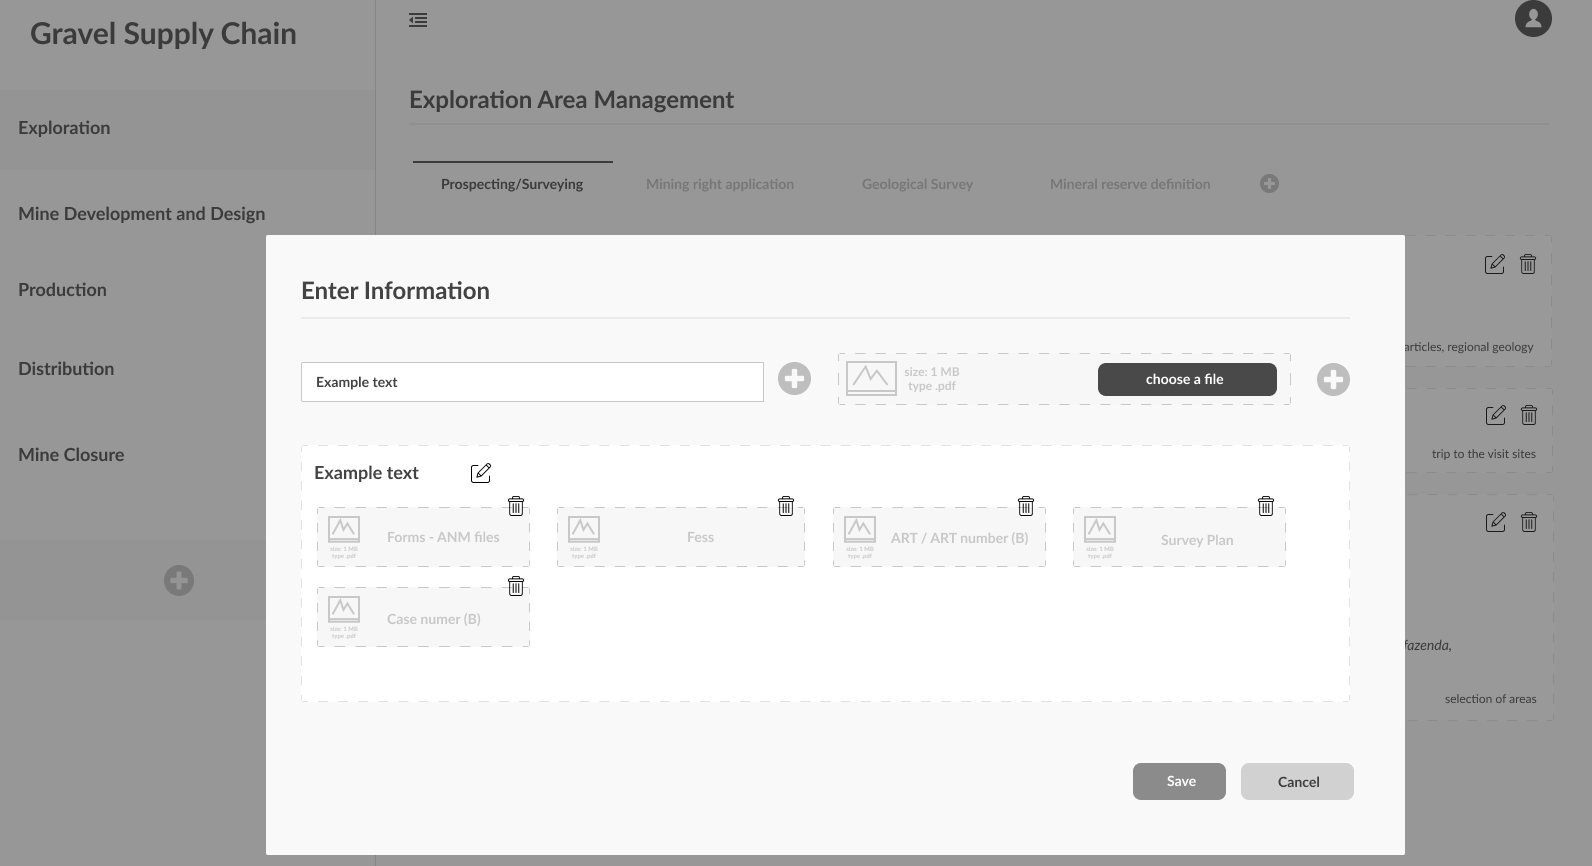
\includegraphics[scale=0.265]{images/frontend02.png}
\caption{SCM Configuration page}
\label{fig:frontend02}
\end{center}
\end{figure*}


Data storage is a general term for archiving data in electromagnetic or other forms for use by a computer or device. Different types of data storage play different roles in a computing environment. In addition to forms of hard data storage, there are now new options for remote data storage, such as cloud computing, and blockchain that can revolutionize the ways that users save and access data.  

Árion uses three applications as data storages: Blockchain, Cloud filesystem and relational database better detailed on next subsections. Blockchains grow continuously because of the amount of data and code in them, which is unchanging. Therefore, an important design decision is to choose which data and calculations to keep in and out of the chain.

\subsubsection{Filesystem}\label{sec:Filesystem}
A cloud file system is a tiered storage system that provides shared access to file data. Users can create, delete, modify, read and write files. All these actions generates a digital fingerprint (hash) information that is stored in the blockchain, separately from the original files or content, to keep consistency, traceability and auditability to the files.

A Cloud file sharing service gives multiple users simultaneous access to a cloud file data set. Cloud file sharing security is managed with user and group permissions, allowing administrators to tightly control access to shared file data.

\subsubsection{Database}\label{sec:Database}
A relational database is a set of formally described tables from which data can be accessed or reassembled in many different ways without having to reorganize the database tables. The standard user and application programming interface (API) of a relational database is the Structured Query Language (SQL). SQL statements are used both for interactive queries for information from a relational database and for gathering data for reports.

\subsubsection{Blockchain}\label{sec:DataStorageBlockchain}
The platform uses Blockchain to supply chain management tracking parts and service provenance, ensuring authenticity of goods, block counterfeits and reducing conflicts. This usually involves a limited and known number of actors, suggesting use of a permissioned Blockchain, that is, a Blockchain where all nodes must be allowed to be part of the system. To implement that, Hyperledger Fabric is used \cite{cachin2016architecture}. Hyperledger is an open source collaborative effort created to advance cross-industry Blockchain technologies. 

Hyperledger Fabric is an enterprise-grade permissioned distributed ledger framework for developing solutions and applications. Its modular and versatile design satisfies a broad range of industry use cases. It offers a unique approach to consensus that enables performance at scale while preserving privacy.

In context of Árion, the Blockchain module consists in smart contracts and the ledger. From the application developer’s perspective, a smart contract, together with the ledger, form the heart of a Hyperledger Fabric Blockchain system. Whereas a ledger holds facts about the current and historical state of a set of business objects, a smart contract defines the executable logic that generates new facts that are added to the ledger. 

\subsubsection{Chaincode}
Hyperledger Fabric implements smart contracts through chaincode. A chaincode is typically used by administrators to group related smart contracts for deployment, but can also be used for low level system programming of Fabric. These terms smart contract and chaincode are used interchangeably in a Hyperledger context. In general, a smart contract defines the transaction logic that controls the lifecycle of a business object contained in the world state. It is then packaged into a chaincode which is then deployed to a Blockchain network. So, smart contracts rule transactions, whereas chaincode rules how smart contracts are packaged for deployment.

Before businesses transact with each other, they must define a common set of contracts covering common terms, data, rules, concept definitions, and processes. Taken together, these contracts lay out the business model that govern all of the interactions between transacting parties. A smart contract defines the rules between different organizations in executable code. Applications invoke a smart contract to generate transactions that are recorded on the ledger.

Smart contracts have many APIs available to them. Critically, in all cases, whether transactions create, read, update or delete business objects in the world state, the Blockchain contains an immutable record of these changes.


\section{Implementation Details} \label{sec:Implementation}

%htbp
\begin{figure*}[ht]
\begin{center}
  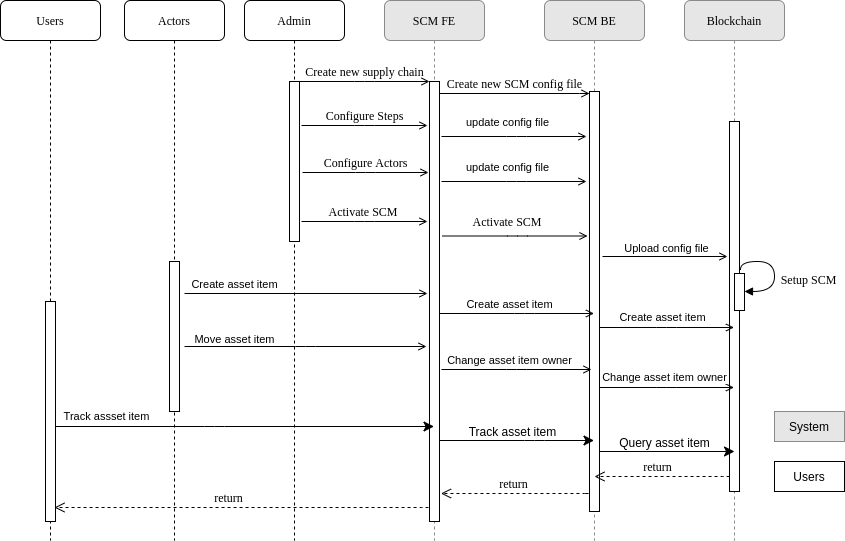
\includegraphics[scale=0.44]{images/SequenceDiagram.png}
\caption{SCM User flow}
\label{fig:sequenceDiagram}
\end{center}
\end{figure*}

Our chaincode is written in Golang and provides all contracts needed to proceed traceability in our application. All contracts for use in chaincode must implement  \textit{contractapi.ContractInterface}. 

The first step is to create a JSON config file providing all information about these three items. A configuration file includes \textit{assetId}, a list of actors and a list of ordered steps. Our chaincode processes this file through  \textit{initLedger} and \textit{createNewAsset} functions. Here follows a template for config file:  

\begin{lstlisting}
{
   "AssetId":"assetName",
   "Actors":[
      {
         "actorType":"type",
         "aditionalInfo":[
            {
               "key":"value"
            }
         ]
      }
   ],
   "Steps":[
      {
         "step":"stepName",
         "stepOrder":1,
         "actorType":"actorType"
      }
   ]
}
\end{lstlisting}

Front-end WebApp enables a user to define settings through a Configuration Page, adding these to the configuration file, as shown in Figure~\ref{fig:frontend02}.

Assets, asset items, steps and actors are described as \textit{structs}. There are create methods for each one,  responsible for create an instance of these \textit{structs} and save the state into the Blockchain. Query methods are responsible for interact with the information of any item in the Blockchain.The function \textit{main} invokes the \textit{initLedger}, reads the configuration files and raises the platform enabling users to interact with the Blockchain via exposing its API. 

When creating an asset item, an \textit{AssetItemId} is generated. Each entity in the chain will have its unique entity ID and timestamp when it starts processing the transaction. By querying \textit{AssetItemId}, the user can easily track the current transaction information and status. Finally, completed all steps, the Blockchain will update \textit{deliverDate} and mark the status as completed once the final actor has received the order. 

\textit{ChangeAssetItemOwner} is the method called to update an asset item when it is moved from a step to another. It updates the \textit{CurrentOwnerId}, the \textit{ProcessDate}, information about prices and many other details of the transactions by the key/value map \textit{  aditionalInfo}. 


The \textit{main} function of chaincode invokes the \textit{initLedger} function, reads the configuration files and raises the platform enabling users to interact with the Blockchain via exposing its API.

Figure~\ref{fig:sequenceDiagram} shows the interaction flow from users with Árion platform. Initially an admin persona creates and configure the SCM adding information about the steps and the users. After that, the admin can activate this SCM and from that point the actors can interact with the SCM to provide information about an asset item and also move this asset item through the supply chain. From that point too, any user can track an asset item to get information about the required good.

\section{Conclusion} \label{sec:Conclusion}

Although, some companies have launched pilot projects using Blockchain technology to manage their supply chains, no detailed information on the technical implementation of such projects has been reported. Either way, the retail industry has the potential to use this technology to improve traceability.  Even if some properties of Blockchain implementation may be useful for supply chain management, there are still a few uses to support this claim. 

In this paper, we proposed a framework for new decentralized traceability systems based on Blockchain technology. This system will deliver online information to all supply chain members on the safety status of goods, providing a more secure, distributed, transparent, and collaborative approach to supply chain management. The framework can significantly improve the development time of Supply Chain Management applications, and provide efficiency and transparency for product management on a supply chain. In a future work, we will present a proof of concept that exercises the use of proposed framework.

%%
%% The next two lines define the bibliography style to be used, and
%% the bibliography file.
\bibliographystyle{ACM-Reference-Format}
\bibliography{sample-base}

%%
%% If your work has an appendix, this is the place to put it.
%\appendix

%\section{Research Methods}

%\subsection{Part One}

\end{document}
\endinput
%%
%% End of file `sample-sigconf.tex'.
